% !TEX root = Main document.tex

 \section{Results and discussion}
\subsection{Torque measurements}
First, the results of the torque measurements single-phase flow are presented and discussed, where drag reduction (DR) is purely the result of a {hydrophobic} surface capturing an air plastron. Second, we show the results for two-phase flow, where air bubbles are added to the flow, that provide bubbly DR and might also add to the stability of the air plastron.
\subsubsection*{Single-phase flow}\noindent
In the top of figure~\ref{fig:DR_delta_nu_Dp_groupplot}, the drag reduction (DR) as defined in equation~(\ref{eq:DR2}) is plotted versus $\Rey$, for the {hydrophobic} inner cylinder (IC) with $\alpha = 0$. This shows an increase in the drag of about \perc{14} over the whole range of $\Rey$ measured. The bottom figure shows the evolution of the thickness of the viscous sublayer ($y^+ = 5$), the viscous length scale and the design parameter suggested by \cite{Park2014} ($y^+ = 1$), and the design parameter suggested by \cite{Bidkar2014} ($y^+ = 0.5$), with the Reynolds number. In figure~\ref{fig:3Re} we show the roughness of the surface expressed in wall units for four different values of $\Rey$: the minimum, the maximum and two intermediate values, for which we use the same data as in figure~\ref{fig:poresize_plot}. For the lowest $\Rey = 0.5 \times 10^6$ , the majority of the roughness length scales is less than $k^+ = 1$ and part of it is even less than $k^+ = 0.5$. However, over the whole range of $\Rey$ measured we find a constant increase of the drag by about $\SI{14}{\%}$. For a rough, wetted surface, an increase of drag with $\Rey$ is expected~\citep{Flack2010}. However, we do not observe wetting of the surface, which would manifest itself through disappearance of the silvery reflection that indicates the presence of an air plastron. Hence, we assume the surface to maintain its Cassie-Baxter state throughout the course of the experiments. \add{Nonetheless, even for a wetted surface, an increase in $C_f$ is very surprising, given the average value of $k^+ < 5$, which would indicate a hydrodynamically smooth surface following~\citep{Schlichting}. A similar result of drag increase with $k^+ < 5$ was also reported by~\cite{Gose2018}. Contrary to the results observed of these authors of increasing DR with decreasing $k^+$ for the same surface, we find a more or less increased constant drag over the whole range of our values of $\Rey$ and hence $k^+$. Our results might be explained by following the analysis of~\cite{Gose2018}, who state that the value of the $k^+$ roughness alone is not sufficient to predict the DR of a superhydrophic surface.} The work of \cite{Reholon2018} showed less DR at larger $\Rey$ due to a thinner and fragmented plastron. However, we find the DR to be more or less constant at $\SI{-14}{\percent}$. \add{When the surface is forced into a wetted state by lowering the surface tension from the addition of TritonX, no significant difference in drag is found. Obviously, the surface roughness strongly influences the drag even in the non-wetted state.}

\begin{figure}
\centering 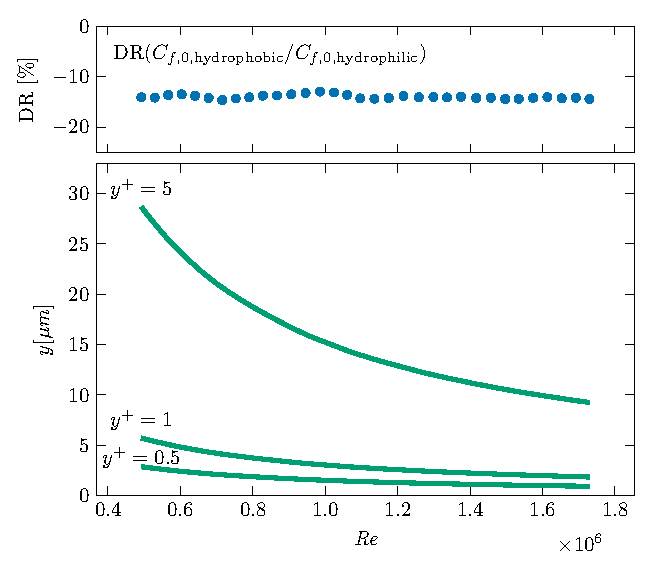
\includegraphics[width=0.76\textwidth]{Figures/fig5}
\caption{Top figure: plot of the drag reduction (DR) as in equation~(\ref{eq:DR2}) versus $\Rey$, with $\alpha = 0$ for the {hydrophobic} inner cylinder. Bottom figure: evolution of the thickness of the viscous sublayer ($y^+ = 5$), the viscous length scale ($y^+ = 1$) and half the viscous length scale ($y^+ = 0.5$) with $\Rey$. The design parameters $w^+ < 1$ and $k^+ < 0.5$ for the {hydrophobic} surface are suggested by \cite{Park2014} and \citep{Bidkar2014} respectively to result in drag reducing behaviour of the surface and are shown here as a reference for the reader. These values are derived from the torque measurements and give therefore an averaged, global value. From figure~\ref{fig:3Re} we find that for our lowest $\Rey$ tested, the majority of the roughness length scales is below $k^+ = 1$ and part of it is below $k^+ = 0.5$. The DR plot however shows a nearly constant increase of the drag by about $\SI{14}{\%}$ over the whole range of $\Rey$ measured.} \label{fig:DR_delta_nu_Dp_groupplot}
\end{figure}

\begin{figure}
\centering 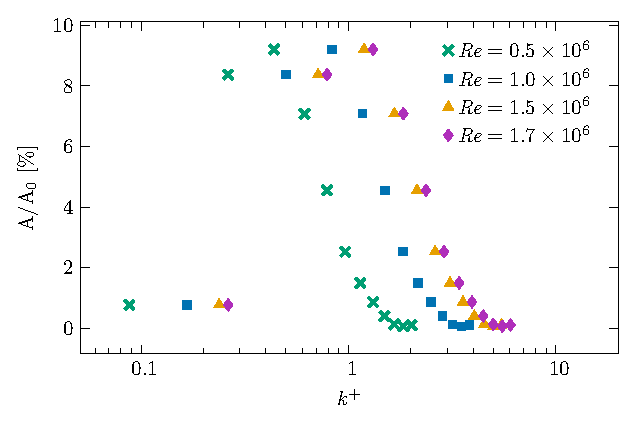
\includegraphics[width=0.8\textwidth]{Figures/fig6}
\caption{Roughness distribution of the surface as coverage fraction of the total area $A/A_0$, expressed in wall units for four different values of $\Rey$. Apart from the maximum and the minimum value of $\Rey$ used in this research, the normalized roughness for two intermediate values of $\Rey$ are shown as well. The wall unit normalization is obtained using data from the torque measurements that gives an averaged, global value of the wall shear stress.} \label{fig:3Re}
\end{figure}


\subsubsection*{Two-phase flow}\noindent
In figure~\ref{fig:DR1}, DR is shown as defined in equation~(\ref{eq:DR1}), comparing results for a \textit{hydrophobic} inner cylinder to a \textit{hydrophilic} inner cylinder, plotted versus $\Rey$. For both hydrophobic and hydrophilic cases, $\alpha = \SI{0}{\percent}$ is the reference case for determining the level of drag reduction that results from the introduction of bubbles ($\alpha > \perc{0}$) to the flow. As an additional effect, the introduction of air bubbles to the working liquid might also lead to enhanced stability of the air plastron~\cite{Lv2014}. With increasing $\Rey$, more DR is found for all measurements. This is in line with the previous findings~\citep{vandenBerg2005,vanGils2013,Spandan2018}. %In in our experiments, $\text{We} = 1$ is reached $\Rey \approx 6 \times 10^5$ and increases with Reynolds number~\citep{vandenBerg2005}.}

Comparing the {hydrophobic} IC to the hydrophilic IC, more bubbly DR is found (figure~\ref{fig:DR1}) over nearly the whole range of $\Rey$  when $\alpha \geq \perc{4}$. Only when $\Rey < 7 \times 10^5$, a slight increase of drag is found for $\alpha = \perc{6}$. In this range of low $\Rey$, the uncertainty of the torque sensor is the highest, as can be seen from the shaded areas in figure~\ref{fig:DR1} that give an indication of the repeatability of the experiments by showing the spread in the data by comparing the extremes of individual measurements. For the smallest amount of air added, $\alpha = \perc{2}$, the {hydrophobic} IC gives more DR compared to the hydrophilic IC up to $\Rey = 10^6$. For larger $\Rey$, between $1.0\times10^6$ and $1.8\times 10^6$, the {hydrophobic} IC gives less DR compared to the hydrophilic IC.

We explain the difference between $\alpha = \perc{2}$ and $\alpha \geq \perc{4}$ in figure~\ref{fig:DR1} as a result of two competing effects: (i) a more effective bubbly drag reduction in the presence of a {hydrophobic} wall, and (ii) a drag increase due to the roughness of this same {hydrophobic} wall. When the thickness of the viscous sublayer $y_\text{vsl} = 5y^+$ decreases with increasing $\Rey$, a larger fraction of the pores on the surface of the {hydrophobic} IC are of a length scale relevant to the flow, as can be seen in figure~\ref{fig:DR_delta_nu_Dp_groupplot}. The balance between these two competing effects determines whether the bubbly DR is more effective when using a rough {hydrophobic} IC compared to a smooth hydrophilic IC. For larger void fractions $\alpha \geq \perc{4}$, the more effective bubbly DR dominates, resulting in more overall DR.

Figure~\ref{fig:deltaDR} shows the difference $\Delta \text{DR}$ between \textit{hydrophobic} and \textit{hydrophilic} from figure~\ref{fig:DR1}, as defined in equation~(\ref{eq:deltaDR}). The difference in $\Delta \text{DR}$ between $\alpha = \perc{4}$ and $\alpha = \perc{6}$ in figure~\ref{fig:deltaDR} is small compared to the difference between $\alpha = \perc{2}$ and $\alpha = \perc{4}$, or $\alpha = \perc{2}$ and $\alpha = \perc{6}$. This suggests that the influence of the {hydrophobic} IC on the bubbly DR is limited, i.e. that a minimum amount of air is required to effectively reduce the drag --- here $\alpha = \perc{4}$ --- but further increasing $\alpha$ will not result in an even stronger influence of the {hydrophobic} IC on the bubbly DR. Nor does $\Delta \text{DR}$ increase with $\Rey$ for $\Rey > 10^6$ and $\alpha \geq \perc{4}$, but rather levels off and starts to decrease. This indicates that of the two effects, the more effective DR from the {hydrophobic} wall initially grows faster with $\Rey$, until $\Delta \text{DR}$ is maximum. With further increasing $\Rey$, around $\Rey = 1.1 \times 10^6$, the balance starts to tilt and the drag increase from the roughness is now the faster growing effect, indicated by the negative slope of $\Delta \text{DR}$ for $\alpha = \perc{4}$ and $\alpha = \perc{6}$ in figure~\ref{fig:deltaDR}. It is tempting to attribute this to wetting of the coating, caused by the wall shear stresses that become larger with $\Rey$. However, if this were the case, a clear difference would be visible between the initial, and its repeated measurements for the same $\alpha$, since the wetted state is the energetically more stable one. It is safe to assume that if the coating -- or part of it -- is wetted, it will not transit back to a non-wetted state between measurements. The reason for the change in balance should therefore be sought elsewhere.

\begin{figure}
\centering 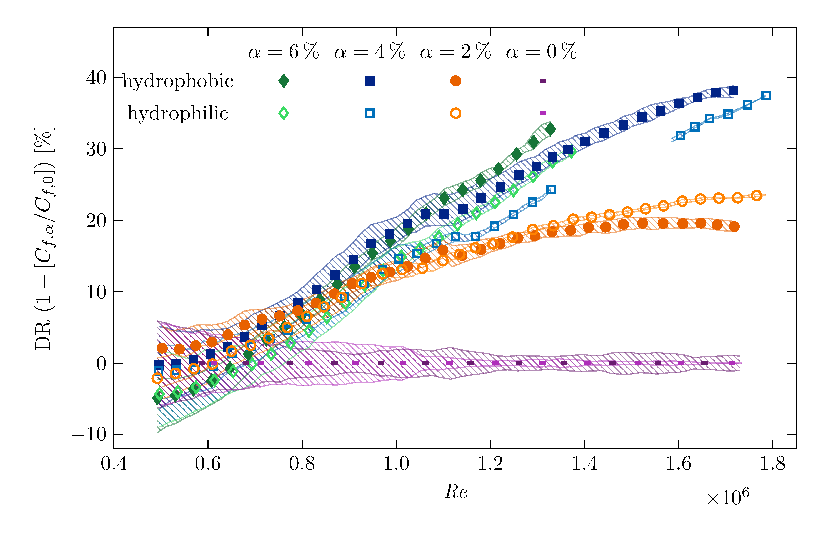
\includegraphics{Figures/fig7}
\caption{Plot of the drag reduction (DR) based on skin friction coefficient $C_f$ as defined in equation~(\ref{eq:DR1}) versus $\Rey$. Compared to figure~\ref{fig:DR2}, is the drag reduction here determined using the same IC as used for the $\alpha > 0$ measurement (so either hydrophobic or hydrophilic) with $\alpha = 0$ ($C_{f,0}$), whereas in figure~\ref{fig:DR2} the reference is the hydrophilic IC with $\alpha = 0$. A more efficient bubbly drag reduction mechanism is found for the hydrophobic coating when the void fraction $\alpha \geq \perc{4}$. For $\alpha  = \perc{2}$ roughness effects dominate, resulting in less overall DR. Only every second data point is shown to improve readability of the plot. The shaded regions represent the spread in data. \add{The size of the error bars based on the accuracy of the torque sensor is smaller than the marker size.} Due to heavy vibrations in the setup resulting from a non-symmetric distribution of air, no data was acquired in the region between $\Rey = 1.3\times10^6$ and $\Rey = 1.6\times10^6$ for $\alpha=\perc{4}$ and for $\Rey > 1.4\times10^6$ when $\alpha=\perc{6}$.}\label{fig:DR1}
\end{figure}



\begin{figure}
\centering
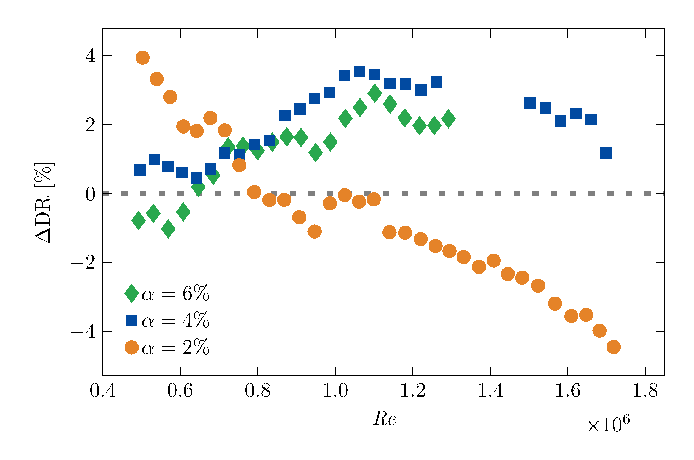
\includegraphics{Figures/fig8}
\caption{Plot of $ \Delta\text{DR} = \text{DR}_\text{hydrophobic} - \text{DR}_\text{hydrophilic}$ from figure~\ref{fig:DR1} versus $\Rey$. For $\alpha = 2$, $\Delta \text{DR}$ decreasing with increasing $\Rey$, owing to the influence of roughness. For $\alpha \geq 4$, $\Delta \text{DR}$ shows an increase with $\Rey$, meaning that the effect of increase in bubbly drag reduction due the hydrophobic coating is stronger than the effect of roughness.}\label{fig:deltaDR}
\end{figure}

The definition of DR$_\text{net}$ in equation~(\ref{eq:DR2}) is used in figure~\ref{fig:DR2} to study the combined effect of both air bubbles ($\alpha > \perc{0}$) and a {hydrophobic} IC, using the hydrophilic IC with $\alpha = \perc{0}$ as a reference for all cases. Compared to figure~\ref{fig:DR1}, all data obtained using the {hydrophobic} IC is shifted downwards by roughly $\perc{15}$.  %Again, a difference is seen between $\alpha \geq \perc{4}$ and $\alpha < \perc{4}$.
For the lines $\alpha = \perc{0}$ and $\alpha = \perc{2}$, the shift in DR$_\text{net}$ is nearly constant, whereas for $\alpha = \perc{4}$ and $\alpha = \perc{6}$ the difference in DR$_\text{net}$ goes down with increasing $\Rey$, owing to the same competing mechanisms as discussed previously. Nonetheless it is clear from figure~\ref{fig:DR2} that for all values of $\alpha$, the use of a {hydrophobic} IC results in a less efficient net DR compared to a hydrophilic IC. The introduction of the {hydrophobic} coating adds roughness to the otherwise hydrodynamically smooth hydrophilic surface, which in this case explains the significant change in the net drag force.

\begin{figure}
\centering 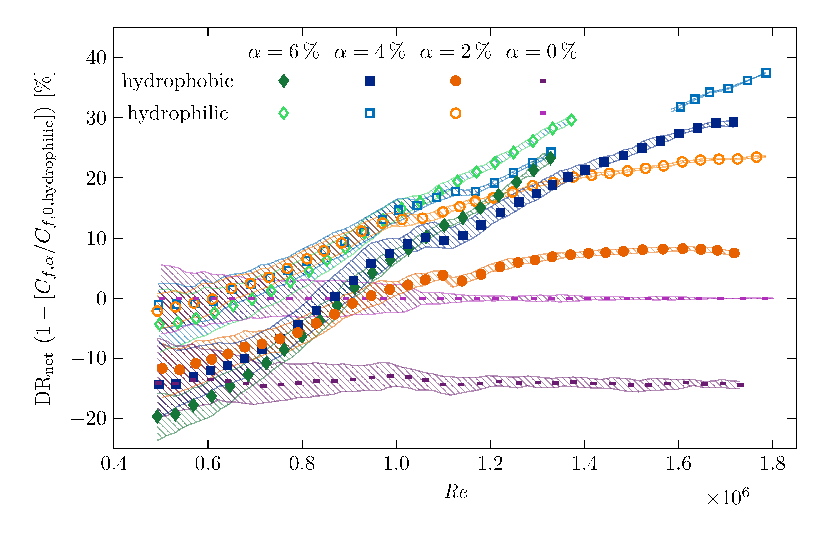
\includegraphics{Figures/fig9}
\caption{Plot of the net drag reduction (DR$_\text{net}$) based on skin friction coefficient $C_f$ (equation~(\ref{eq:DR2})) versus $\Rey$. Compared to figure~\ref{fig:DR1}, is the drag reduction here determined using the hydrophilic IC with $\alpha = 0$ as the reference ($C_{f,0,\text{hydrophilic}}$), whereas in figure~\ref{fig:DR1} the reference is the same IC as used for the $\alpha > 0$ measurement (so either hydrophobic or hydrophilic) with $\alpha = 0$.  For all values of $\alpha$, the use of the coating results in less efficient net DR compared to an uncoated cylinder. Only every second data point is shown to improve readability of the plot. The shaded regions represent the spread in data. \add{The size of the error bars based on the accuracy of the torque sensor is smaller than the marker size.} Due to heavy vibrations in the setup resulting from a non-symmetric distribution of air, no data was acquired in the region between $\Rey = 1.3\times10^6$ and $\Rey = 1.6\times10^6$ for $\alpha=\perc{4}$ and for $\Rey > 1.4\times10^6$ when $\alpha=\perc{6}$.}\label{fig:DR2}
\end{figure}


\subsection{Repeatability and measurement errors of torque measurements}
For the highest Reynolds number achieved in this research, namely $\Rey = 1.8\times10^6$, the shear stress at the surface $\tau_w = \mathcal{T} / 2 \pi r_i^2 L_\text{mid}$ is \SI{274}{\Pa}. To ensure that the {hydrophobic} coating applied to the IC is not adversely affected by this high shear stress, we measured the $\alpha = \perc{0}$ reference measurement twice after every series of $\alpha > \perc{0}$ measurements, as indicated in table~\ref{table:measurement_order}. The skin friction coefficients found in the $\alpha = \perc{0}$ measurements have a spread of \perc{3}. This spread shows no trend, which suggests that the properties of the coating remain constant throughout the experiments. This was also confirmed by visual inspection of the coating and by comparison of SEM images of the coating taken before and after the measurements.  \\
The repeated measurements of $\alpha = \perc{2}, \perc{4}, \text{and } \perc{6}$ show a spread in skin friction coefficient of $\perc{2}, \perc{4}, \text{and } \perc{2}$, respectively, again suggesting good measurement repeatability. \add{The accuracy of the torque sensor is rated by the manufacturer to be $\pm \perc{0.25}$ of its maximum rated output. Error regression analysis has shown that the largest error in figures~\ref{fig:DR1}~and~\ref{fig:DR2} is slightly smaller than the markers used.} The data spread is reflected by the shaded regions in figures~\ref{fig:DR1}~and~\ref{fig:DR2}. These regions are derived by using the minimum and maximum values from the repeated measurements for $C_{f,0}$ and $C_{f,\alpha}$.

\subsection{Velocity profiles}
Shown in figure~\ref{fig:PIVplot} are the results on the velocity profiles from the PIV measurements. Plotted are the azimuthal velocities normalized with the velocity of the inner cylinder $u_\theta / u_i$, versus the normalized position between the inner and outer cylinder $(r - r_i) / d$, for different Reynolds numbers. We compare the \textit{hydrophilic} IC to the \textit{hydrophobic} IC, for a single-phase flow with $\alpha = \perc{0}$. A clear difference is seen in the region close to the IC, with larger velocities for the {hydrophobic} IC compared to the hydrophilic IC at similar Reynolds numbers. This is attributed to the larger roughness of the {hydrophobic} IC compared to the hydrophilic IC. A rougher surface can transport more energy to the flow compared to a smooth surface, resulting in larger velocities in the near wall region for the same driving of the flow~\citep{Zhu2018}. In other flow configurations, when the wall is not used to drive the flow, lower velocities will be found for more rough surfaces~\citep{Flack2010,MacDonald2016,Busse2017}. For larger $\Rey$ we find larger velocities close to the IC, indicating that the effect of the roughness is stronger with larger $\Rey$. This reflects the reduction in thickness of the viscous sublayer, which results in a larger fraction of the small scale roughness (pores) of the {hydrophobic} IC becoming a relevant length scale to the flow.

\begin{figure}
\centering 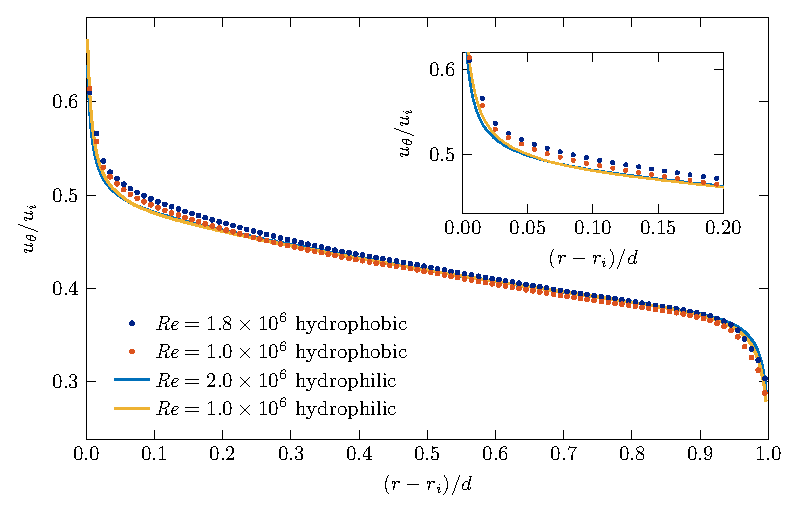
\includegraphics{Figures/fig10} \caption{Plot of azimuthal velocity normalized with inner cylinder velocity $u_\theta / u_i$ versus the normalized gap width between inner and outer cylinder $(r-r_i) / d$. The working fluid is without air, so $\alpha = \perc{0}$. Compared is the rough \textit{hydrophobic} coating with the smooth \textit{hydrophilic} steel inner cylinder. The \textit{hydrophilic} data is provided by~\cite{hui13} using the same experimental setup. The inset shows the region close to the inner cylinder. }\label{fig:PIVplot}
\end{figure}
